\chapter{\textbf{Experimental Setup}}
Wireless sensor networks (WSNs) are networks of interconnected wireless devices that are embedded into the physical environment to provide measurements of many points over large spaces. These devices have built-in processing, storage, and radio frequency sensors and antennas. They are linked into an interconnected network that routes the data they capture to a computer for analysis.\\
Environmental protection is one of the most challenging tasks for humanity. All of the latest technologies to certain extent are applied in this area, among others, wireless sensor networks as well. In this paper a wireless sensor node designed specifically for monitoring of environmental parameters is described. The main advantage of this node is the use of energy harvesting techniques and supercapacitor as power supply method. The absence of batteries affects the reduction of maintenance costs and environmental impact. The paper shows that combination of energy harvesting and supercapacitor represents a sustainable solution of constant power supply of wireless sensor network node.
The WSN has one or more sensor node. These sensor nodes are used to extract data from the environment of the home. A Router is used to develop local IP based web server. It will provide a muscular networking mechanism over comfortable range of Wireless sensor areas over local IP. The wireless sensor node is consisting of ESP8266 Wi-Fi module, sensors and actuators. A webserver is designed for user interface to monitor the sensor data and control the node operation and actuation state.\\\\
In this chapter the detailed implementation of the proposed system is aggregated. The main structures that are needed to be developed for home automation are the Implementation and design of
\begin{enumerate}
\item	WSN
\item Server gateway
\item Local server
\item Web interface
\end{enumerate}
The WSN has one or more sensor node. These sensor nodes are used to extract data from the environment of the home.
\clearpage
\section{Implementation of sensor-based node}
A wireless sensor node is a popular solution when it is difficult or impossible to run a mains supply to the sensor node. However, since the wireless sensor node is often placed in a hard-to-reach location, changing the battery regularly can be costly and inconvenient. An important aspect in the development of a wireless sensor node is ensuring that there is always adequate energy available to power the system.The ESP8266 humidity-temperature sensor node uses the Digital Humidity and Temperature (DHT11) sensor, which is connected to the ESP8266 modules’ GPIO pin 0. DHT11 sensor is used to collect the raw humidity and temperature data. It is a basic temperature and capacitive humidity sensor which works on 3-5 V power. The sensor node has a wireless connection with a router where the router works as a gateway in the star topology network.\\\\
\begin{figure}[H]
  \centering
  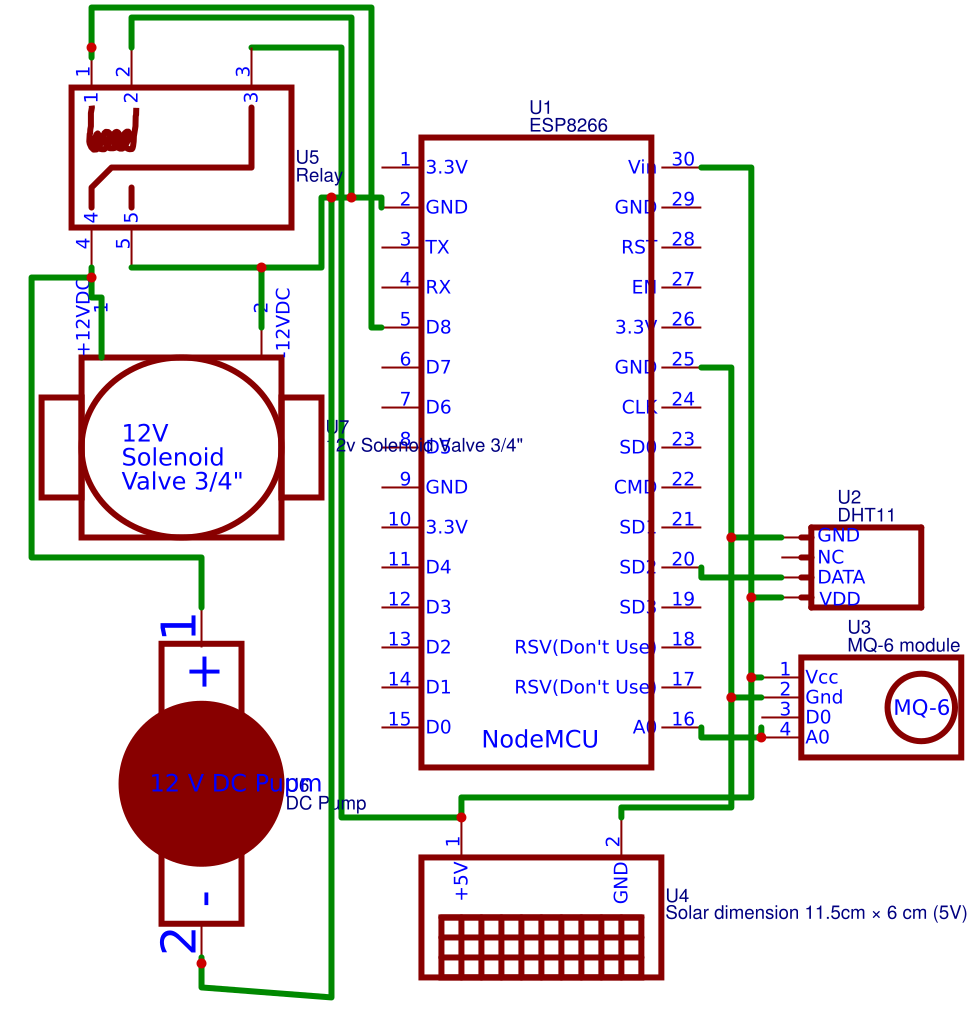
\includegraphics[width=5in]{35}
  \caption{Schematic Diagram of the System}\label{fig35}
\end{figure}
The gas sensor node is used for the monitoring and enhancing the kitchen safety of the home. The schematic and wiring diagram are presented in Figure 6.1. The DIO pin of MQ-2 is connected to the ESP8266 DIO pin 0. The other connections are same as temperature and humidity sensor node.\\

\section{Implementation of solar panel}
The ESP8266 is powered by the 3.7V battery that is connected to the Solar Lipo Charger in the battery input port. The solar cells are connected in the PWR In ports. The Vin and GND ports of the ESP8266 are connected to Vout ports of the Solar Lipo Charger.\\\\
The BME280 power is supplied by the 3.3V port in the ESP8266. The communication is done through the I2C lines (SDA / SCL). For the sleep mode, D0 need to be connected to reset pin (RST). To fix all components in the box, a preboard is used.
\begin{figure}[H]
  \centering
  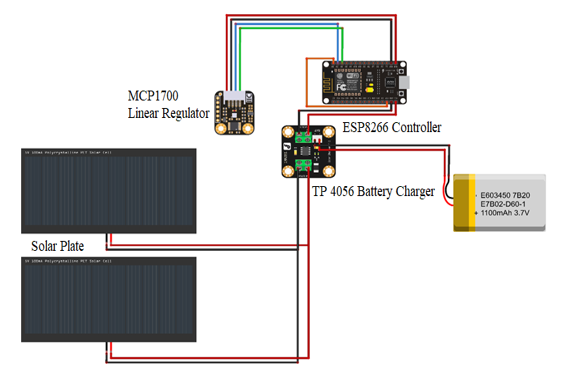
\includegraphics[width=6in]{36}
  \caption{Schematic diagram of a solar panel}\label{fig36}
\end{figure}
\section{Data Acquisition and Storage}
The software service running on the server performs the following two tasks:
\begin{enumerate}
  \item acquiring the data
  \item storing the data.
\end{enumerate}
A TCP socket receives sensor data created by the gateway in the form of TCP packets. Once a UDP packet is received, the sample data is extracted from the payload, and the source address of the ESP8266 Module that sent the data is extracted from the IPv6 source address of the TCP packet. The second task is to create a database for sensor sample extracted from the TCP packet using the information extracted from a TCP packet.\\
\begin{figure}[h]
  \centering
  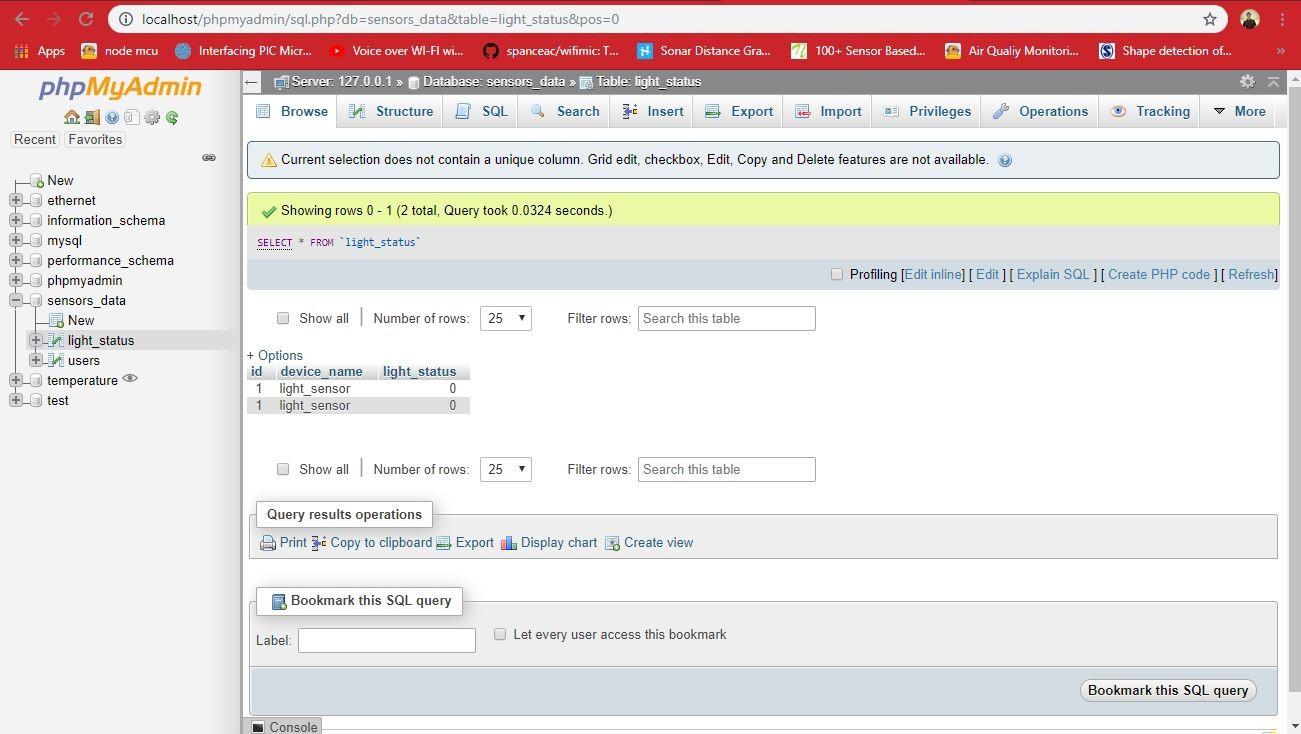
\includegraphics[width=6in]{39}
  \caption{Database Server (PHP my admin).}\label{fig39}
\end{figure}
\subsection{Database Server}
For hosting a website in the local machine XAMPP software package is used. Raspberry pi
works as a local server machine in which XAMPP package is installed. It facilitates in hosting website and works as a local database server. The software package also contains Apache MySQL server. The MySQL server is used to create database for the proposed system which is shown in Fig. 4.7. In MySQL server, data acquired by sensors are stored and retrieved when needed. Also, information’s of the end user are stored in the database. For the administration of the created database from remote panel PhpMyAdmin is also configured.
\begin{enumerate}
  \item Sensor ID
  \item Sensor Channel
  \item Date and time
  \item Sample Data
\end{enumerate}
When user sends a get request via the web interface PHP converts it into MySQL queries. PHP establishes the connection to the MySQL server and then fetch or post data according to the user command. The fetched data is then sent back to the html webpage for showing it to the user. HTML works in the client side for getting and PHP works in the server side for handling request for client. When the raspberry pi is powered and connected to the internet, the webpage hosted in it can be accessed from anywhere of the world. The sensor data from the TCP packet is stored in a MySQL database in an organized way. These sensors data are stored with a designated sensor ID, sensor channel and date and time in MySQL database so that the designed webpage can access those data.The data stored in the database can be viewed in the webpage.

\subsection{Receiving Data Samples}
The basic network communication between two programs is defined as socket. It is the endpoint of a two-way communication link. In an OS, the socket has two operating mode, client and server. When the OS acts as a client it is connected to the server to exchange data through the socket. In server mode the socket listens for incoming connections from clients. A socket is bound to a port number so that the TCP layer can identify the application that data is destined to be sent to. An endpoint is a combination of an IP address and a port number.\\
Data can be fetched from MySQL tables by executing SQL SELECT statement through PHP function mysql query.Several options are required to fetch data from MySQL.The most frequently used option is to use function mysql fetch array.
\begin{figure}[H]
  \centering
  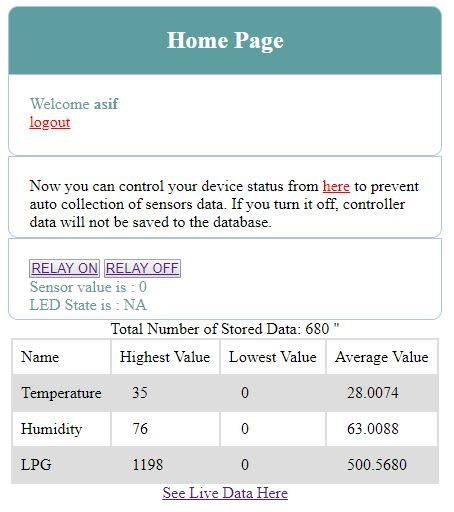
\includegraphics[width=4in]{38}
  \caption{Highest and lowest data samples. }\label{fig38}
\end{figure}



\section{ Web Interface}
The website in the server which is used to control the digital output pins is a group of pages
on World Wide Web containing buttons, sliders, sensors data and User Interface (UI) allowing the user to control the appliances all over the world through HTTP protocols. The webpage interface is used for controlling appliances, equipment like light, fan, cooler, air-conditioner etc. The status of different equipment is also visualized in the webpage. The developed webpage is presented in Figure-6.6.
\begin{figure}[H]
  \centering
  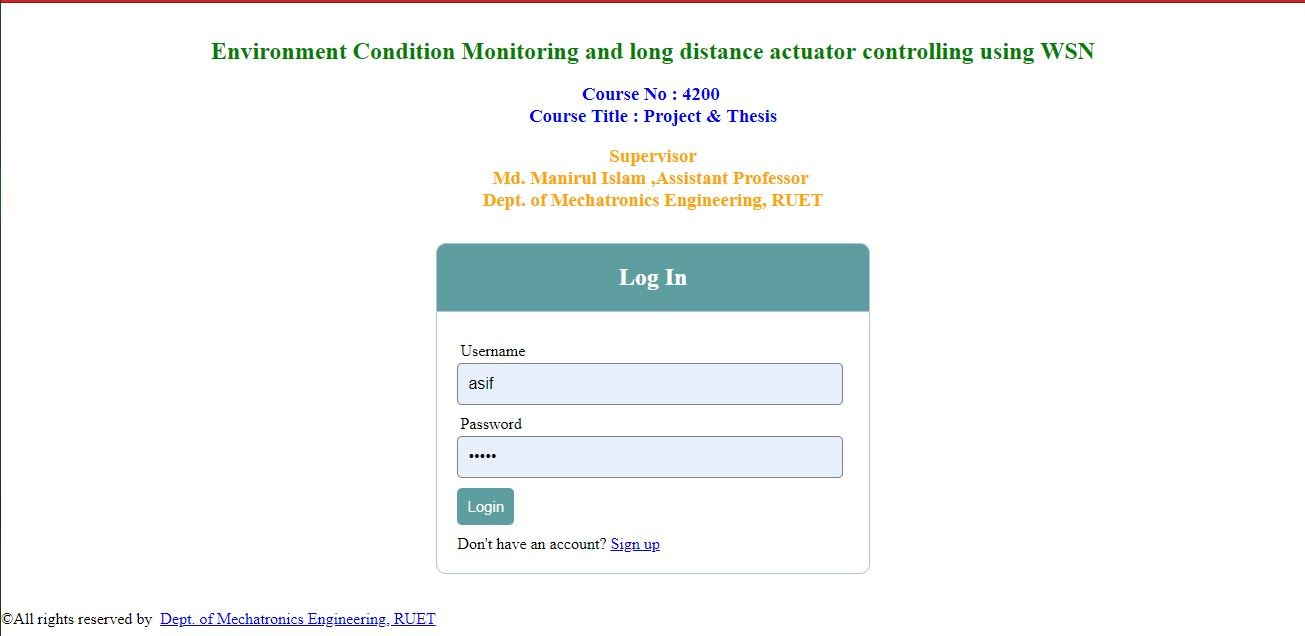
\includegraphics[width=6in]{40}
  \caption{Web interface}\label{fig40}
\end{figure}
Html files, .txt file and PHP files comprise the website to store data and to control the things by toggling the current state of the digital output pins. The web interface for the client side is implemented using HTML, CSS, JavaScript, Ajax, jQuery, and PHP script. The static web page is designed using HTML and CSS. CSS is a language that describes the style and elements of an HTML document. This static page is not interactive to user. To make it dynamic and interactive to the end user JavaScript is used for client-side scripting. jQuery is used to simplify the programing of JavaScript. It is a widely-used JavaScript library. Ajax is used as an interface language between client-side web applications and a server. It is a for user group of interrelated Web development techniques which is used on the client side to create asynchronous web applications. With Ajax, client-side web application can exchange data and status of the GPIO pin with a server asynchronously in the background without interfering with the display and behavior of the existing page. To continuously extract data from the MySQL data base A PHP script is written.
\section{Retrieving Data from Database}
To retrieve data from database the sensor id, sensor channel, and data and time range are required. These parameters are used to create a SQL query to the database to retrieve the required sensor samples. A PHP script is written which contains those database parameters to generate a SQL query for the purpose of retrieving data. These data are placed on JSON array. The output of the JSON array are then transferred to the web browser. The web browser calls the PHP scripts to retrieve data by running a java script. For the control of GPIO pins another PHP script which toggles the current state of the GPIO pins is also called by the web page to generate a control message when graphical interface buttons, sliders are operated.Although records are normally retrieved in the order in which they are inserted into the database, data cannot rely on a particular order being preserved. If created database was backed up and restored, or if a maintenance operation was performed on the database, MySQL might alter the order in which records were stored internally.
\begin{figure}[H]
  \centering
  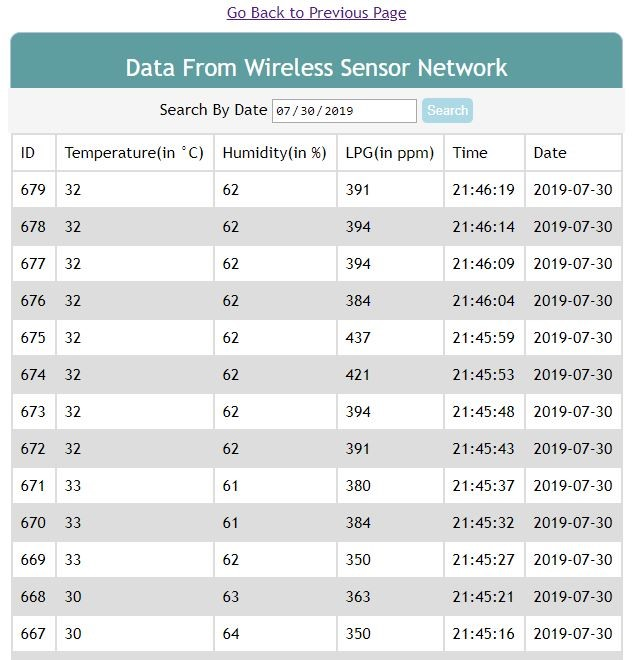
\includegraphics[width=4in]{37}
  \caption{Data stored in database.}\label{fig37}
\end{figure}
\section{Controlling actuator from the web server}
To take you one step ahead towards WSN development, today we will make our own web server to host a webpage and control any appliance remotely from anywhere in the world. Here ESP12E NodeMCU was used as webserver, although any ESP module can be used here.\\\\
In simple terms, Web server is a place where we can store the web pages, process them and deliver them to the web clients. A protocol is used to establish and transfer information between web client and server. This protocol is known as Hypertext Transfer Protocol (HTTP). In this protocol, communication is initiated by making a request for a particular web page using HTTP GET request and the server responds with the content of that web page. If server does not respond it will through an error message i.e. 404 Error. Webpages delivered by the server are mostly in HTML coding.
\begin{figure}[H]
  \centering
  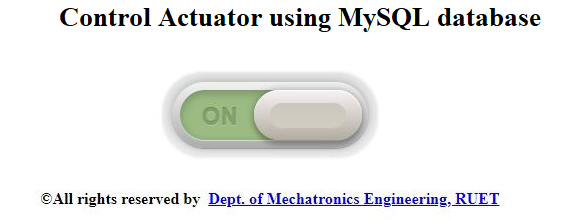
\includegraphics[width=6in]{42}
  \caption{Controlling Actuator from server }\label{fig42}
\end{figure}
All the websites are hosted on some webserver, mostly Linux based operating system is used on webservers. Any computer can be converted into a webserver, provided that it is connected to the network. We have previously done many webserver projects with different microcontrollers. Raspberry pi already has inbuilt Wi-Fi module so it doesn't need any other hardware to turn it into a webserver, whereas other microcontroller needs some network connecter (ESP module) for a webserver.
\section{Final Setup}
Final setup of the project was made by the components described earlier.The setup outlook was made by using PVC board and all the components were calibrated before installation.The system performance was satisfactory.
\begin{figure}[H]
  \centering
  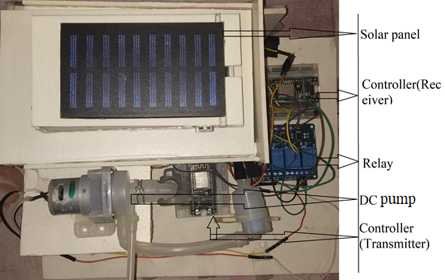
\includegraphics[width=4in]{44}
  \caption{Implemented system  }\label{fig44}
\end{figure}
The relay was also did the satisfactory level performance.The system was under a trial about 1 hour randomly.In trial period the relay control state wasn't show any error.The Figure 6.9 represent the relay state with respect to time.
\begin{figure}[h]
  \centering
  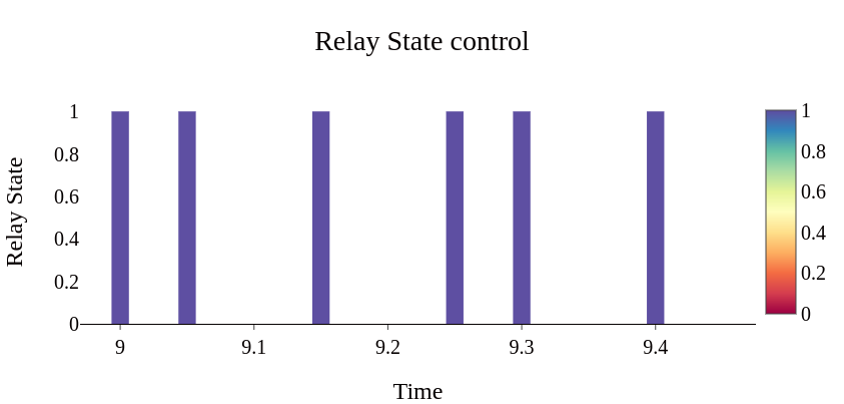
\includegraphics[width=4 in]{47}
  \caption{Relay state ON/OFF using Feedforward \& Feedback control system (For Actuator Controlling}\label{fig46}
\end{figure}

\section{Chapter Summery}
In this Chapter the experimental setup is described along with the database which was created for the WSN sensor node.This chapter in this volume have presented the best available knowledge of database and some of technologies and tools available for this setup.The objectives of the chapter is to apply this knowledge in the development of the WSN node and the database for storing the data alongside for controlling the Actuator.  